% arara: pdflatex: {shell: true}
\documentclass[a4paper]{article}
\usepackage{latexsym,amssymb,amsmath,amsbsy,amsopn,amstext,xcolor,multicol}
\usepackage{ctex,hyperref,graphicx,wrapfig,fancybox,listings,subfigure}
\usepackage[top=1in, bottom=1in, left=1.25in, right=1.25in]{geometry}
\graphicspath{{fig/}}

\usepackage{color}
 
\definecolor{codegreen}{rgb}{0,0.6,0}
\definecolor{codegray}{rgb}{0.5,0.5,0.5}
\definecolor{codepurple}{rgb}{0.58,0,0.82}
\definecolor{backcolour}{rgb}{0.95,0.95,0.92}
 
\lstdefinestyle{mystyle}{
    backgroundcolor=\color{backcolour},   
    commentstyle=\color{codegreen},
    keywordstyle=\color{magenta},
    numberstyle=\tiny\color{codegray},
    stringstyle=\color{codepurple},
    basicstyle=\footnotesize,
    breakatwhitespace=false,         
    breaklines=true,                 
    captionpos=b,                    
    keepspaces=true,                 
    numbers=left,                    
    numbersep=5pt,                  
    showspaces=false,                
    showstringspaces=false,
    showtabs=false,                  
    tabsize=2
}
 
\lstset{style=mystyle}
\renewcommand{\figurename}{图}
\title{\bf 数字图像处理作业报告}
\date{2019.4}
\author{英62~~王怡力~2016012642}
\begin{document}
\kaishu
\ttfamily
\maketitle
\tableofcontents
\newpage
\section{Poisson Image Editting}
\subsection{测试环境}

本程序在macOS High Sierra 10.13.6 环境下编译。测试前请使用命令 
\texttt{pip install -r requirements.txt --user}安装第三方库 \underline{\textbf{opencv}}, \underline{\textbf{scipy}} 和\underline{\textbf{numpy}}。可直接在命令行输入\texttt{python3 ./main.py}运行demo,运行结果保存在\texttt{./test/}文件夹内

\subsection{Mask UI}


本程序默认的输入只有source和target两张图(提前做作业导致以为不会给mask), 因此我首先实现的是交互式的Mask生成器。我调用了opencv里自带的User Interface函数, 生成了两个可供用户交互的界面 --- Mask painter and Mask mover。Mask painter可让用户自己选择想要融合的部分

\begin{figure}[htpb]
  \centering 
  \subfigure[界面一]{ 
    %\label{fig:subfig:a} %% label for first subfigure 
    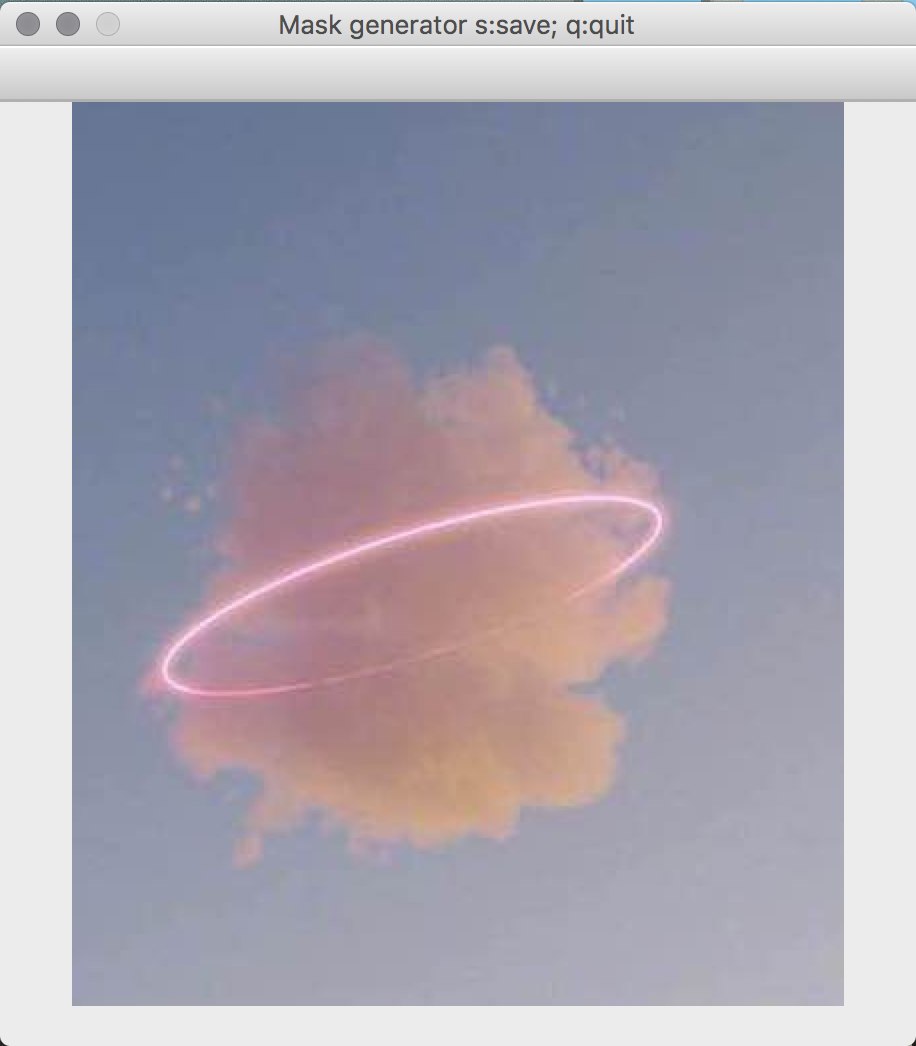
\includegraphics[width=1.5in]{fig/painter-1.png} 
  } 
  \subfigure[框选融合区域]{ 
    %\label{fig:subfig:b} %% label for second subfigure 
    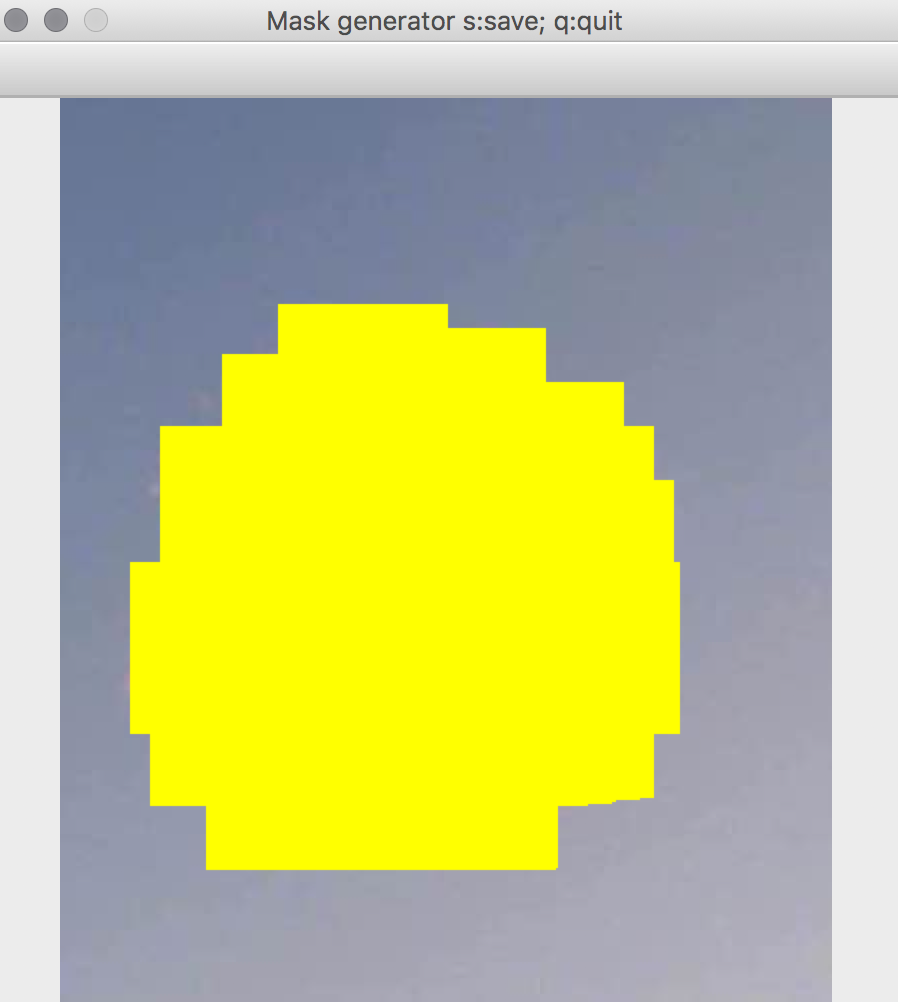
\includegraphics[width=1.5in]{fig/painter-2.png} 
  } 
  %\label{fig:subfig} %% label for entire figure 
\end{figure}

点按 \texttt{s} 保存之后,第二个界面会自动跳出,Mask mover 可让用户确定融合部分在目标图片中的放置区域:

\begin{figure}[htpb]
  \centering 
  \subfigure[界面二]{ 
    %\label{fig:subfig:a} %% label for first subfigure 
    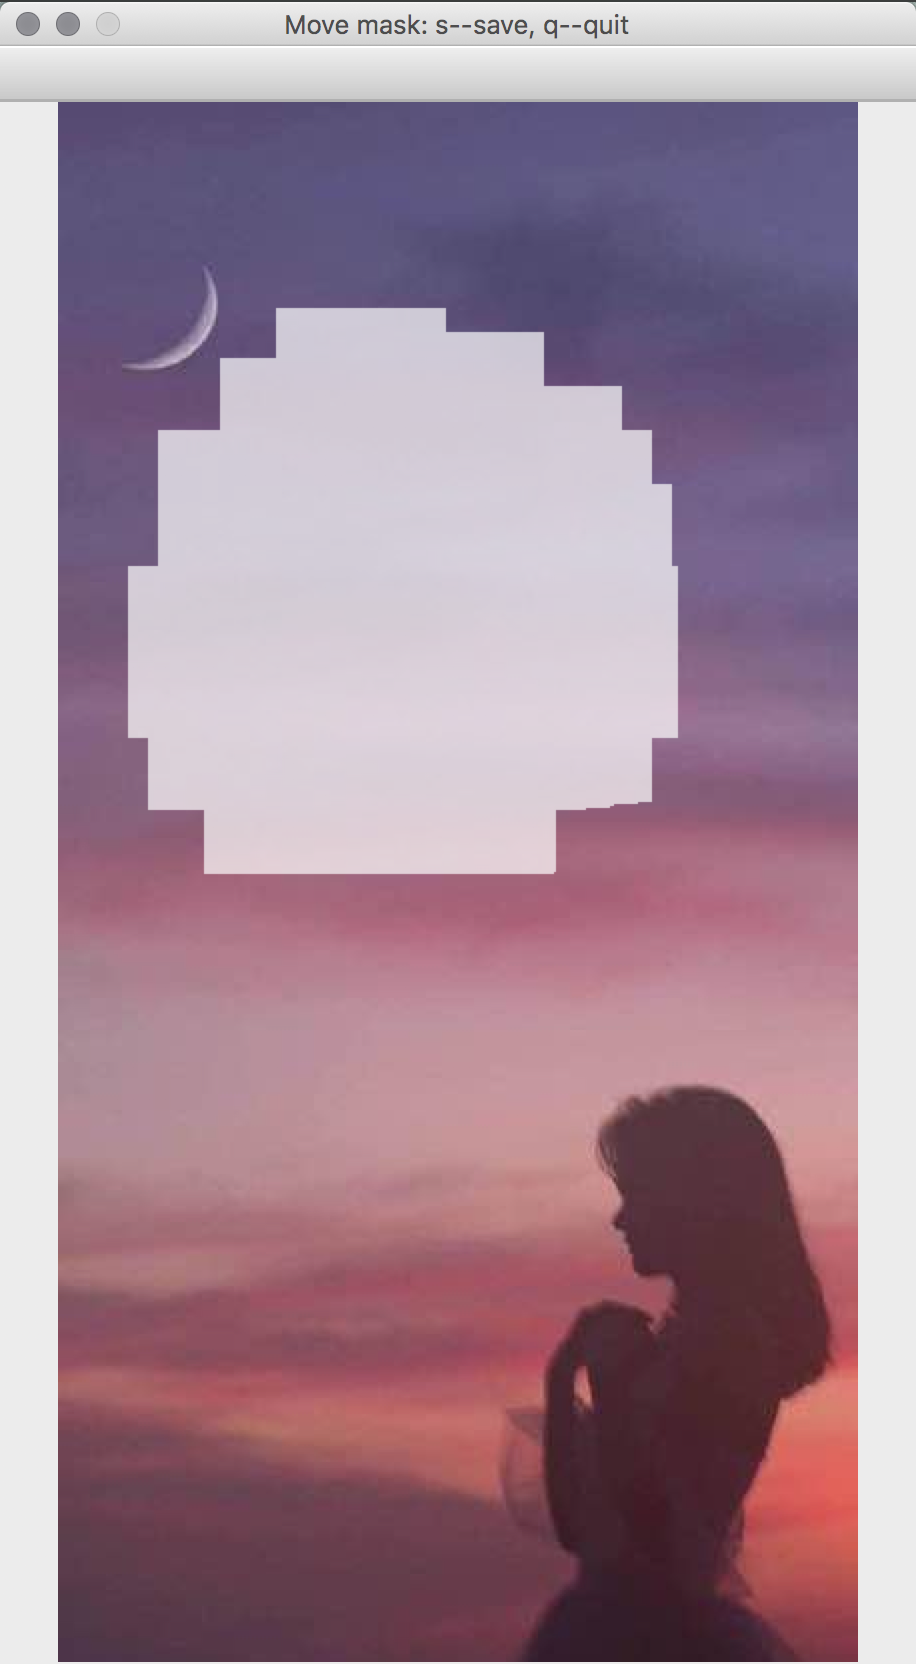
\includegraphics[width=1.2in]{fig/mover-1.png} 
  } 
  \subfigure[移动融合区域]{ 
    %\label{fig:subfig:b} %% label for second subfigure 
    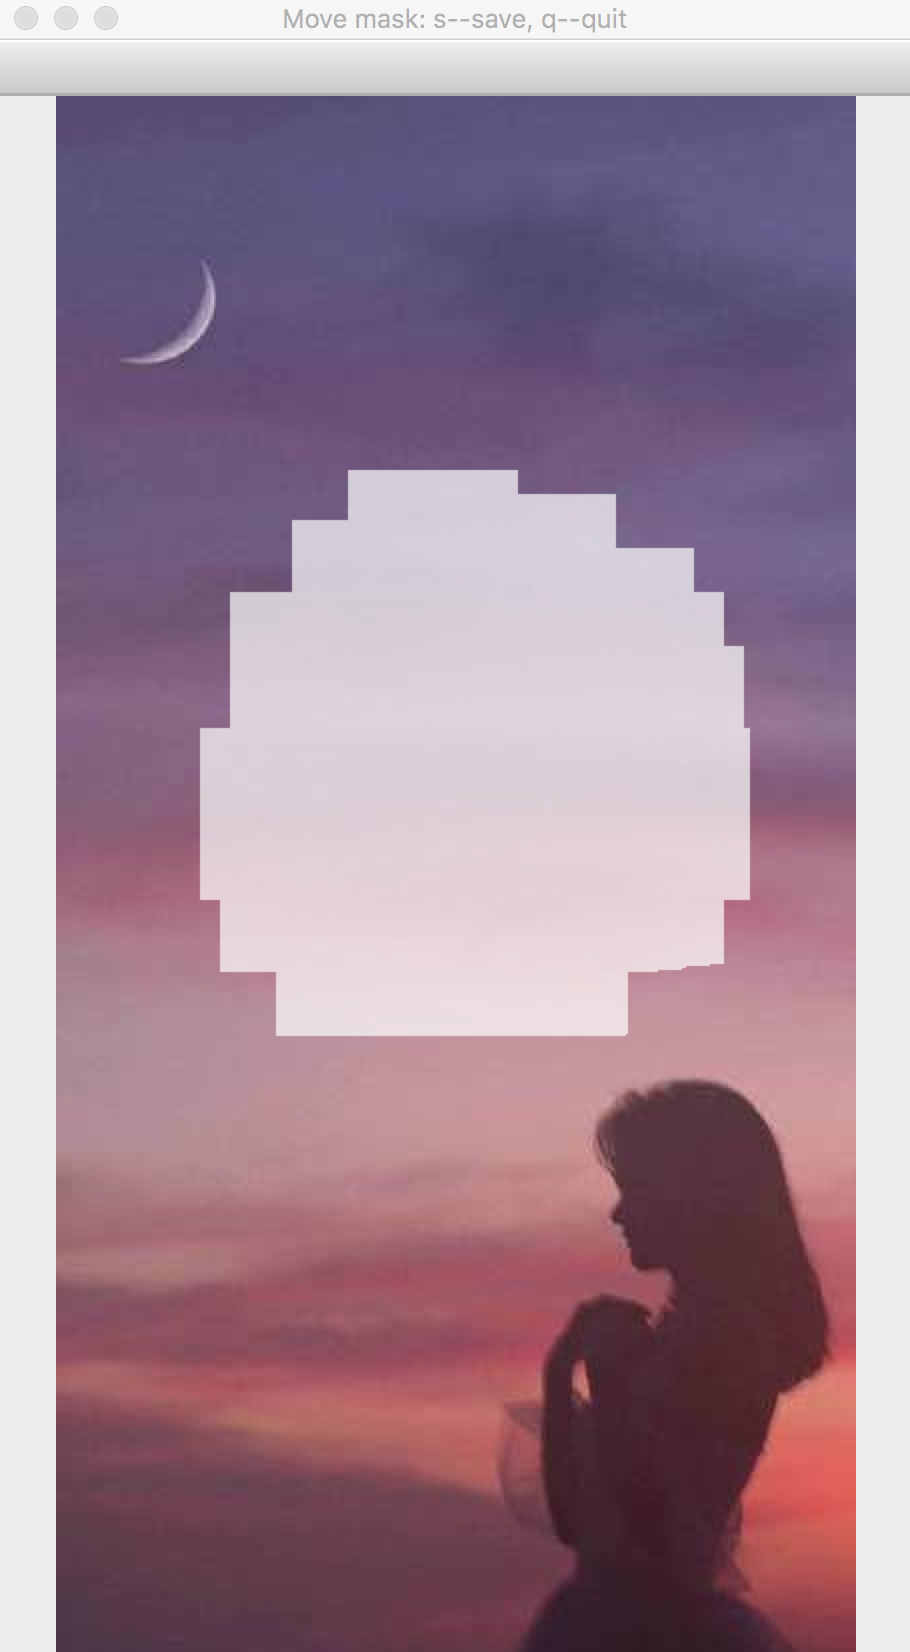
\includegraphics[width=1.2in]{fig/mover-2.png} 
  } 
  %\label{fig:subfig} %% label for entire figure 
\end{figure}

最后Mask UI会在原图像目录下输出喂给泊松融合的标准source,mask图片,这两张图片和target尺寸大小相等,且source待融合区域的位置与target对应

\begin{figure}[htpb]
  \centering 
   \subfigure[目标图像]{ 
    %\label{fig:subfig:a} %% label for first subfigure 
    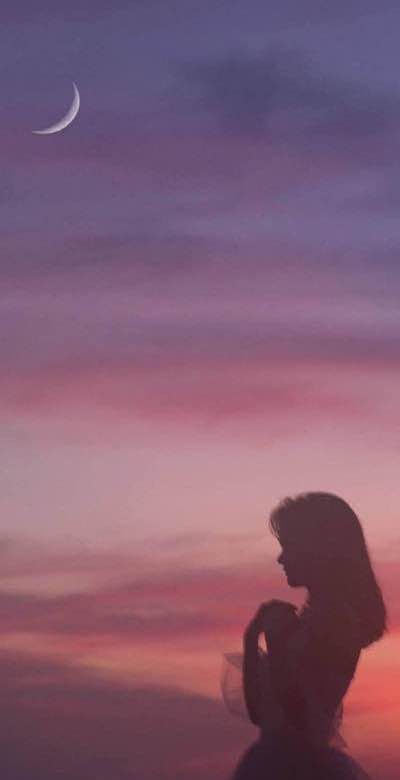
\includegraphics[width=1.2in]{fig/target.png} 
  } 
  \subfigure[标准化原图像]{ 
    %\label{fig:subfig:a} %% label for first subfigure 
    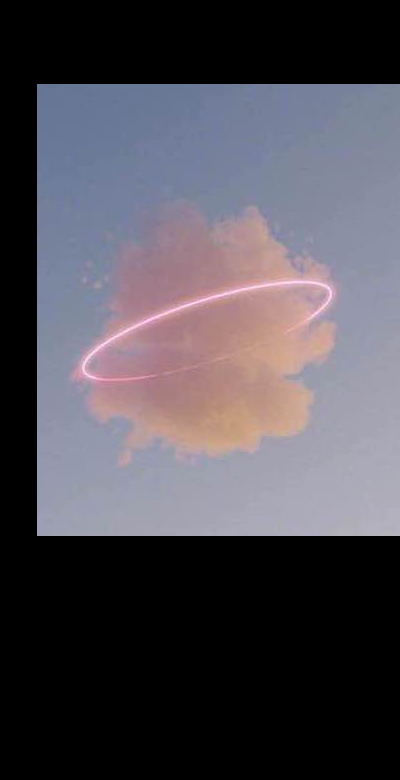
\includegraphics[width=1.2in]{fig/transformed_source.png} 
  } 
  \subfigure[标准化Mask]{ 
    %\label{fig:subfig:b} %% label for second subfigure 
    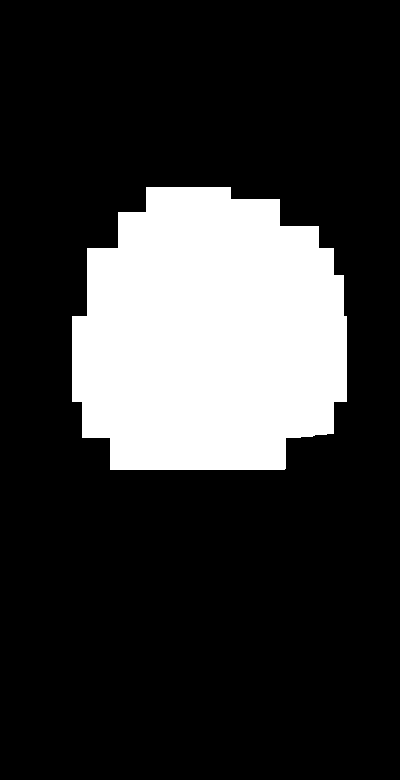
\includegraphics[width=1.2in]{fig/transformed_mask.png} 
  } 
  \subfigure[处理后]{ 
    %\label{fig:subfig:b} %% label for second subfigure 
    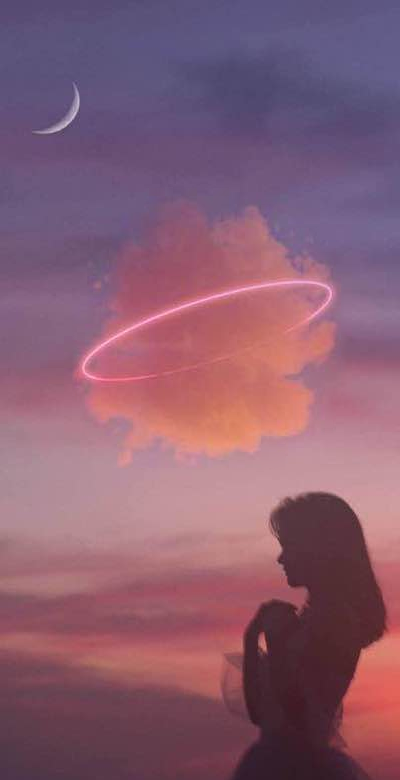
\includegraphics[width=1.2in]{fig/result3.png} 
  } 
  %\label{fig:subfig} %% label for entire figure 
\end{figure}




\subsection{Poisson Edit}

\subsubsection{问题描述}
给出目标图片$T(x,y)$,原图片$S(x,y)$, 我们要让融合部分的图像内部$\Omega$的梯度尽可能的接近原图像$S(x,y)$,同时融合部分图像的边界$\partial\Omega$需要满足边界条件$I(x,y) = T(x,y) \ on \ \partial \Omega$。问题可被形式化的表达为
$$\min_{I(x,y)\in \Omega} \int\int_{\Omega}\|\nabla I(x,y) - \nabla S(x,y)\|^2 dxdy\ \ s.t. \ \ I(x,y) = T(x,y)\ \  \forall(x,y)\in \partial \Omega$$


\subsubsection{方程表示}
问题的本质是解一个泊松方程
$$\nabla^2I(x,y) = \nabla^2S(x,y) \in \Omega$$$$ I(x,y) = T(x,y) \in \partial \Omega $$
我们分情况去考虑这个问题,对于一个在$\Omega$里的像素$p$, 若其周围的像素都在内部,则由$\nabla^2I(x,y) = \nabla^2S(x,y) \in \Omega$,对其进行离散的近似求解,将拉普拉斯算子作用在这个像素上,我们可以得到
\begin{align}
I(x+1,y)& +I(x-1,y) + I(x,y-1)+I(x,y+1)-4I(x,y)  \\
&= S(x+1,y)+S(x-1,y) + S(x,y-1)+S(x,y+1)-4S(x,y) 
\end{align}
对于一个在$\Omega$里的像素$p$,若其周围存在像素位于$\partial \Omega$,假设其为$(x,y+1)$和$(x,y-1)$ 我们有
\begin{align}
I(x+1,y)& +I(x-1,y) + T(x,y-1)+T(x,y+1)-4I(x,y)  \\
&= S(x+1,y)+S(x-1,y) + S(x,y-1)+S(x,y+1)-4S(x,y) 
\end{align}

联立这些方程我们可以得到一个线性系统 $A\vec{i} = b$,$A$是一个巨大的稀疏矩阵,每一行最多有五个非零元,且对角线上的元素均为4.$b$是由$S's$和$T's$构成的。

构造出方程等式的核心代码如下

\begin{lstlisting}[language=Python]
#get spare matrix A
def sparse_mat(points):
    num = len(points)
    A = lil_matrix((num,num))
    for i,index in enumerate(points):
        A[i,i] = 4
        for p in get_neighbor(index):
            if p in points: 
                j = points.index(p)
                A[i,j] = -1
    A = lil_matrix.tocsc(A)
    return A
#get vector b 
def calculate_vec(points,source,target):
    num = len(points)
    b = np.zeros(num)
    for i,index in enumerate(points):
        x,y = index
        b[i] = (4 * source[x,y])- 1*source[x+1, y] - 1*source[x-1, y]- 1*source[x, y+1] -  1*source[x, y-1]
        if on_boundary(index,points):
            for p in get_neighbor(index):
                if p not in points:
                    b[i] += target[p]
    return b
\end{lstlisting}

\subsubsection{方程求解}

考虑到这是一个维数非常大的矩阵,对于稀疏线性系统,本程序使用了针对稀疏线性系统的迭代方法$Jacobi$,$Gauss-Seidel$和$successive over-relaxation (SOR) $求解。

\begin{itemize}
\item \textbf{$Jacobi$}

第$i^{th}$行等式可以表示为
\begin{align}
&a_{ii} x_i = b_i -\sum_{j<i} a_{ij}x_j -\sum_{j>i} a_{ij}x_i\\
&x_i = ( b_i -\sum_{j<i} a_{ij}x_j -\sum_{j>i} a_{ij}x_i)/a_{ii}
\end{align}
算法可描述为,迭代直到收敛
\begin{align}x_i^{k+1} = ( b_i -\sum_{j<i} a_{ij}x_j^{k} -\sum_{j>i} a_{ij}x_i^{k})/a_{ii}\end{align}
\item \textbf{$Gauss-Seidel$}

$Gauss-Seidel$仅仅是将等式右边第二个迭代项修改为$x_j^{k+1}$
\begin{align}x_i^{k+1} = ( b_i -\sum_{j<i} a_{ij}x_j^{k+1} -\sum_{j>i} a_{ij}x_i^{k})/a_{ii}\end{align}
\item \textbf{$SOR$}

$successive\ over-relaxation$ 在$Gauss-Seidel$的基础上加入了松弛项,一般有更快的收敛速度
\begin{align}x_i^{k+1} = (1-\omega)x_i^{k} + \frac{\omega}{a_{ii}}( b_i -\sum_{j<i} a_{ij}x_j^{k+1} -\sum_{j>i} a_{ij}x_i^{k})/a_{ii}
\end{align}
$Jacobi$,$Gauss-Seidel$和$successive over-relaxation (SOR) $写成矩阵的形式,有 $A = L + D + U$,$L$为$A$的下对角元素矩阵,$D$为$A$的对角元素矩阵,$U$为$A$的上对角元素矩阵

$Jacobi$ 
$$M x^{k+1} = Nx^{k} + b $$
其中 $M = D, N_J = -(L+U)$

$Gauss-Seidel$
$$M x^{k+1} = Nx^{k} + b $$
其中 $M = D+L, N_J = -U$

$successive over-relaxation (SOR) $
$$(D+\omega L) x^{k+1} = \omega b - [\omega U + (\omega -1)D]x^{k} $$

核心代码如下

\begin{lstlisting}[language=Python]
if option.lower() == 'jacobi':
		w= 1
		M = sp.spdiags(extract_diag(A),0,np.size(A,0),np.size(A,1))
		N = M-A
	elif option.lower() == 'gauss':
		w = 1
		M = sp.tril(A,0)
		N = M-A
	elif option.lower() == 'sor':
		w= 1
		diaV = extract_diag(A)
		M = sp.spdiags(diaV,0,np.size(A,0),np.size(A,1))+w*sp.tril(A,-1)
		N = (1-w)*sp.spdiags(diaV,0,np.size(A,0),np.size(A,1))-w*sp.triu(A,1)
\end{lstlisting}

\end{itemize}


\subsection{效果}
\subsubsection{融合效果}
\begin{figure}[htpb]
  \centering 
  \subfigure[目标图像]{ 
    %\label{fig:subfig:a} %% label for first subfigure 
    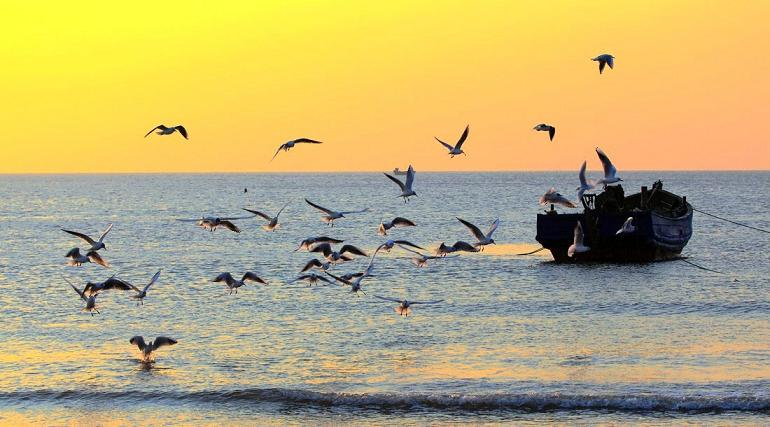
\includegraphics[width=2.5in]{fig/target1.png} 
  } 
  \subfigure[处理后]{ 
    %\label{fig:subfig:b} %% label for second subfigure 
    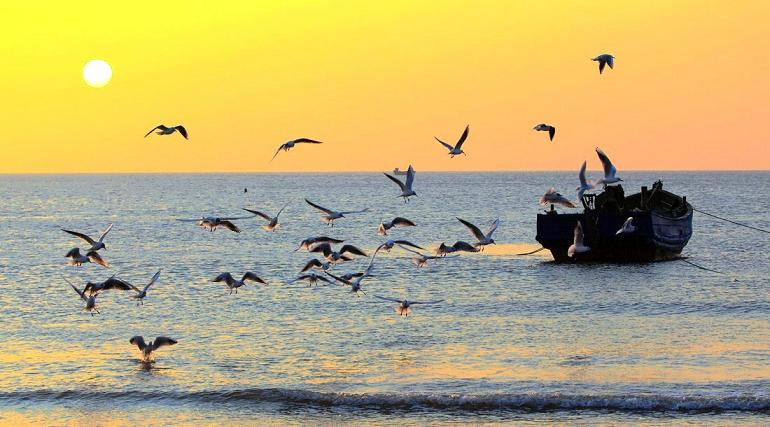
\includegraphics[width=2.5in]{fig/result1.png} 
  } 
  %\label{fig:subfig} %% label for entire figure 
\end{figure}

\begin{figure}[htpb]
  \centering 
  \subfigure[目标图像]{ 
    %\label{fig:subfig:a} %% label for first subfigure 
    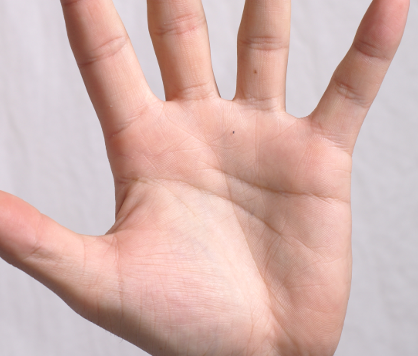
\includegraphics[width=2.5in]{fig/target2.png} 
  } 
  \subfigure[处理后]{ 
    %\label{fig:subfig:b} %% label for second subfigure 
    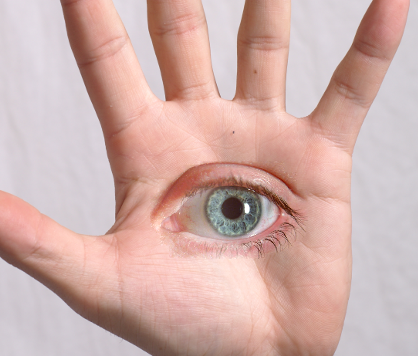
\includegraphics[width=2.5in]{fig/result2.png} 
  } 
  %\label{fig:subfig} %% label for entire figure 
\end{figure}


\subsubsection{迭代效果}

以下是Jacobi和Gauss-Seidel迭代方法迭代50次,200次,1000次,2500次,5000次的效果(report/fig/文件夹里也有sor的效果,但由于和gauss-sneil没有显著区别,就没有放在报告里了)
在迭代速度上,Jacobi方法明显慢于Gauss-Seidel方法. 动画效果见demo.gif

\begin{figure}[htpb]
  \centering 
  \subfigure[Jacobi,50]{ 
    %\label{fig:subfig:a} %% label for first subfigure 
    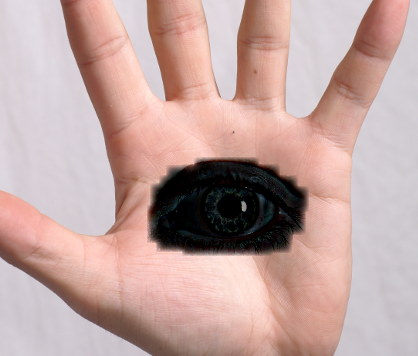
\includegraphics[width=2.0in]{fig/50-jacobi.png} 
  } 
  \subfigure[Gauss-Seidel,50]{ 
    %\label{fig:subfig:b} %% label for second subfigure 
    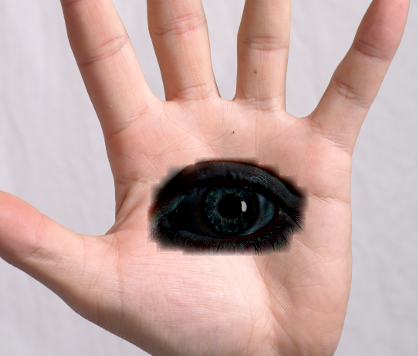
\includegraphics[width=2.0in]{fig/50-gauss.png} 
  } 
\end{figure}


\begin{figure}[htpb]
  \centering 
  \subfigure[Jacobi,200]{ 
    %\label{fig:subfig:a} %% label for first subfigure 
    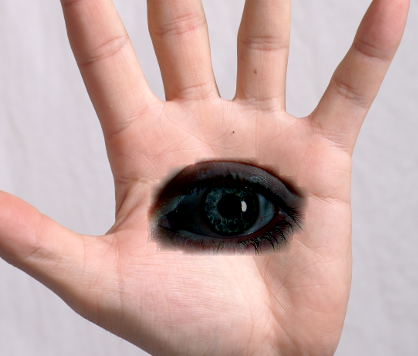
\includegraphics[width=2.0in]{fig/200-jacobi.png} 
  } 
  \subfigure[Gauss-Seidel,200]{ 
    %\label{fig:subfig:b} %% label for second subfigure 
    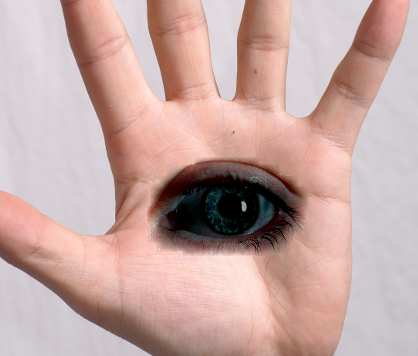
\includegraphics[width=2.0in]{fig/200-gauss.png} 
  } 
\end{figure}
\begin{figure}[htpb]
  \centering 
  \subfigure[Jacobi,1000]{ 
    %\label{fig:subfig:a} %% label for first subfigure 
    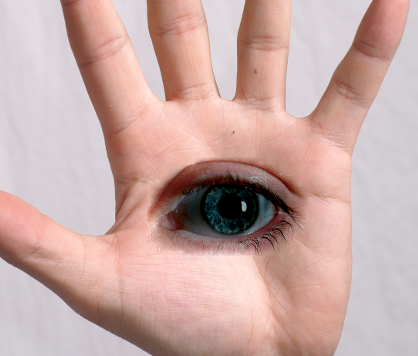
\includegraphics[width=2.0in]{fig/1000-jacobi.png} 
  } 
  \subfigure[Gauss-Seidel,1000]{ 
    %\label{fig:subfig:b} %% label for second subfigure 
    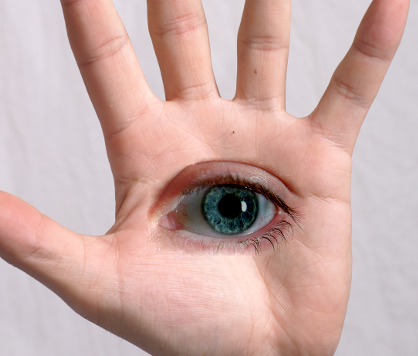
\includegraphics[width=2.0in]{fig/1000-gauss.png} 
  } 
\end{figure}
\begin{figure}[htpb]
  \centering 
  \subfigure[Jacobi,2500]{ 
    %\label{fig:subfig:a} %% label for first subfigure 
    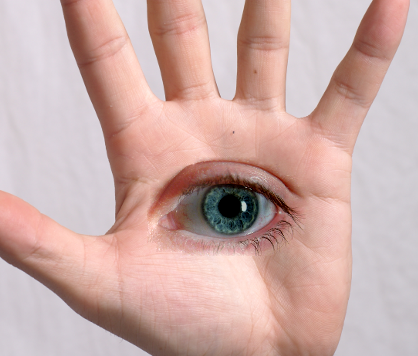
\includegraphics[width=2.0in]{fig/2500-jacobi.png} 
  } 
  \subfigure[Gauss-Seidel,2500]{ 
    %\label{fig:subfig:b} %% label for second subfigure 
    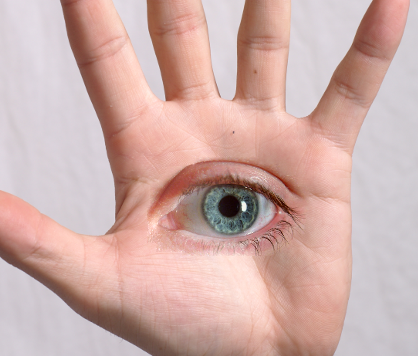
\includegraphics[width=2.0in]{fig/2500-gauss.png} 
  } 
\end{figure}
\begin{figure}[htpb]
  \centering 
  \subfigure[Jacobi,5000]{ 
    %\label{fig:subfig:a} %% label for first subfigure 
    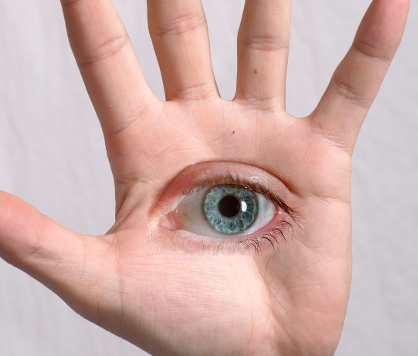
\includegraphics[width=2.0in]{fig/5000-jacobi.png} 
  } 
  \subfigure[Gauss-Seidel,5000]{ 
    %\label{fig:subfig:b} %% label for second subfigure 
    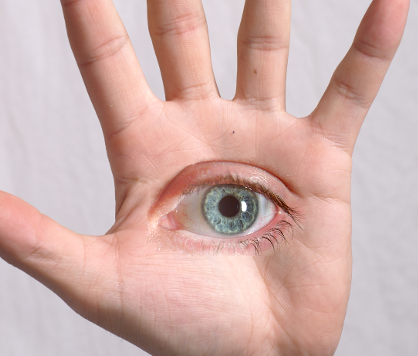
\includegraphics[width=2.0in]{fig/5000-gauss.png} 
  } 
\end{figure}

\end{document}
